% LaTeX path to the root directory of the current project, from the directory in which this file resides
% and path to econtexPaths which defines the rest of the paths like \FigDir
\providecommand{\econtexRoot}{}\renewcommand{\econtexRoot}{.}
\providecommand{\econtexPaths}{}\renewcommand{\econtexPaths}{\econtexRoot/Resources/econtexPaths}
% The \commands below are required to allow sharing of the same base code via Github between TeXLive on a local machine and Overleaf (which is a proxy for "a standard distribution of LaTeX").  This is an ugly solution to the requirement that custom LaTeX packages be accessible, and that Overleaf prohibits symbolic links
\providecommand{\econtex}{\econtexRoot/Resources/texmf-local/tex/latex/econtex}
\providecommand{\econtexSetup}{\econtexRoot/Resources/texmf-local/tex/latex/econtexSetup}
\providecommand{\econtexShortcuts}{\econtexRoot/Resources/texmf-local/tex/latex/econtexShortcuts}
\providecommand{\econtexBibMake}{\econtexRoot/Resources/texmf-local/tex/latex/econtexBibMake}
\providecommand{\econtexBibStyle}{\econtexRoot/Resources/texmf-local/bibtex/bst/econtex}
\providecommand{\econtexBib}{economics}
\providecommand{\notes}{\econtexRoot/Resources/texmf-local/tex/latex/handout}
\providecommand{\handoutSetup}{\econtexRoot/Resources/texmf-local/tex/latex/handoutSetup}
\providecommand{\handoutShortcuts}{\econtexRoot/Resources/texmf-local/tex/latex/handoutShortcuts}
\providecommand{\handoutBibMake}{\econtexRoot/Resources/texmf-local/tex/latex/handoutBibMake}
\providecommand{\handoutBibStyle}{\econtexRoot/Resources/texmf-local/bibtex/bst/handout}

\providecommand{\FigDir}{\econtexRoot/Figures}
\providecommand{\CodeDir}{\econtexRoot/Code}
\providecommand{\DataDir}{\econtexRoot/Data}
\providecommand{\SlideDir}{\econtexRoot/Slides}
\providecommand{\TableDir}{\econtexRoot/Tables}
\providecommand{\ApndxDir}{\econtexRoot/Appendices}

\providecommand{\ResourcesDir}{\econtexRoot/Resources}
\providecommand{\rootFromOut}{..} % Path back to root directory from output-directory
\providecommand{\LaTeXGenerated}{\econtexRoot/LaTeX} % Put generated files in subdirectory
\providecommand{\econtexPaths}{\econtexRoot/Resources/econtexPaths}
\providecommand{\LaTeXInputs}{\econtexRoot/Resources/LaTeXInputs}
\providecommand{\LtxDir}{LaTeX/}
\providecommand{\EqDir}{Equations} % Put generated files in subdirectory

\documentclass[pdflatex]{beamer}
\providecommand{\texname}{ProjectMMD-Slides}% Indicate the keyname for the bibtex entry corresponding to this document
\providecommand{\texnameMaster}{ProjectMMD}% Indicate the keyname for the bibtex entry corresponding to this document
\newif\ifdvi\dvifalse

%\usepackage{optional}
\usepackage{ifthen}%\usepackage{\econtexRoot/BufferStockTeory}

% Can't read in ProjectMMD.sty because some packages conflict with Beamer
% So need to redefine everything here

\usepackage{\econtexShortcuts}
\usepackage{natbib,amsmath,amssymb,rotating,subfigure}
\usepackage{verbatim,moreverb,graphicx}
\usepackage{wasysym}
\usepackage{dcolumn}
\usepackage{cancel}
\usepackage{booktabs}
% \providecommand{\LtxDir\EqDir}{\econtexRoot/Equations}
\providecommand{\FigsRaw}{\econtexRoot/Code/Python/Figures}
\providecommand{\CodeDir}{\econtexRoot/Code}
\providecommand{\CalibrationDir}{\econtexRoot/Calibration}
\providecommand{\TableDir}{\econtexRoot/Tables}
\providecommand{\ApndxDir}{\econtexRoot/Appendices}
\providecommand{\Ex}{\mathbb{E}}

%\usepackage{natbib}\newcommand*{\newblock}{}

\mode<presentation>
{
  \usetheme{Warsaw}
  % or ...
  \setbeamercovered{transparent}
}

%\beamerdefaultoverlayspecification{<+->}

%\setbeamertemplate{navigation symbols}{}  % Take away navigation symbols

\usetheme{Warsaw}

\setbeamersize{text margin left=3mm}
\setbeamersize{text margin right=3mm}


%_____________ Opening slide _______________________

\title[Project MMD]{A Simple Labor-Leisure Model with Habits: Some Simulations from Previous Results}
\author[Drozd]{Mark M. Drozd}
\institute[JHU]{Johns Hopkins University}
\date[\today]{December 7, 2021}

\begin{document}\bibliographystyle{\econtexBibStyle}

\begin{frame}[plain]
  \titlepage
\end{frame}


%_____________ 1st section  ____________
\section{Introduction}
\subsection{Motivation}

\begin{frame}
\frametitle{Introduction}

\begin{itemize}
\item Introduce habits into the life-cycle labor supply model
  \begin{itemize}
  \item Already has been done (see \cite{bover1991relaxing})
  \end{itemize}
\item Use the previous results to create some visualizations
  \item Change the parameter values to assess the validity of the model. 
\item Even under perfect foresight, this problem is fairly tough.
  \end{itemize}
\end{frame}

\begin{frame}
  \frametitle{Key Result}
\begin{itemize}
\item Original point estimates for the parameter values too high
  \begin{itemize}
  \item Risk-free rate in the 20\% range (if only this were true!)
  \end{itemize}
 \item Adjustment of wage elasticities.
\end{itemize}
\end{frame}

%______________2nd section__________________
\section{The Problem}
\begin{frame}
\frametitle{The Problem}
\end{frame}


\begin{frame}
  \frametitle{Overview--Pictorially}
  \begin{figure}[ht]
  \centerline{
    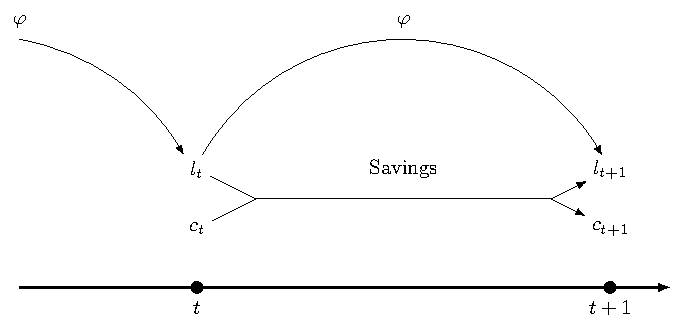
\includegraphics[width=3.5in]{\FigDir/stylized_model}
  }
  \caption{Stylized Model} \label{fig:stylized_model}
  \footnotesize{Behold a stylized model of the labor-leisure model with habits.}
\end{figure}




  \end{frame}

% _____________3rd Section____________________
\section{Simulations}

\begin{frame}
  \frametitle{Calibrations}
  \begin{table}
\centering
\caption{Calibrated Parameters}
\label{tab:calibs}
\begin{tabular}{lrrrrr}
\toprule
{} & $\gamma_h$ & $\gamma_c$ & $\varphi$ & $\rho$ &      r \\
Simulation     &            &            &           &        &        \\
\midrule
Original       &  1768.1516 &  4454.0084 &    0.2205 & 0.2429 & 0.2429 \\
Realistic      &  1768.1516 &  4454.0084 &    0.2205 & 0.0800 & 0.0200 \\
Counterfactual &  1768.1516 &  4454.0084 &    0.1000 & 0.0800 & 0.0200 \\
\bottomrule
\end{tabular}
\end{table}

  \end{frame}

  \begin{frame}
    \frametitle{Life Cycle Consumption}
    \begin{center}
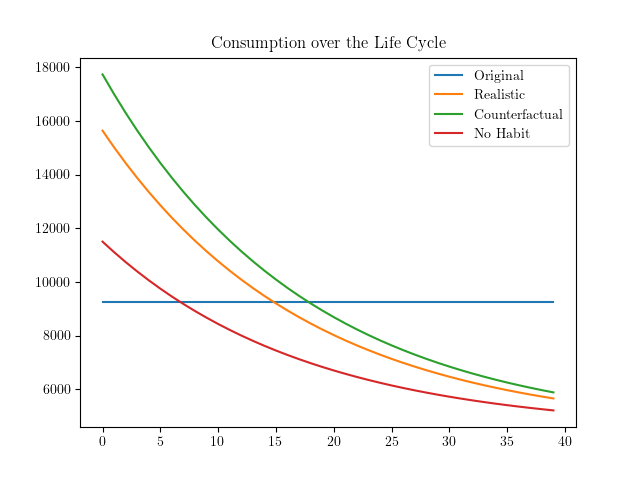
\includegraphics[width=0.8\textwidth]{\FigDir/consumption_lc.png}
\end{center}
\end{frame}

    \begin{frame}
      \frametitle{Life Cycle Labor Hours}
      \begin{center}
      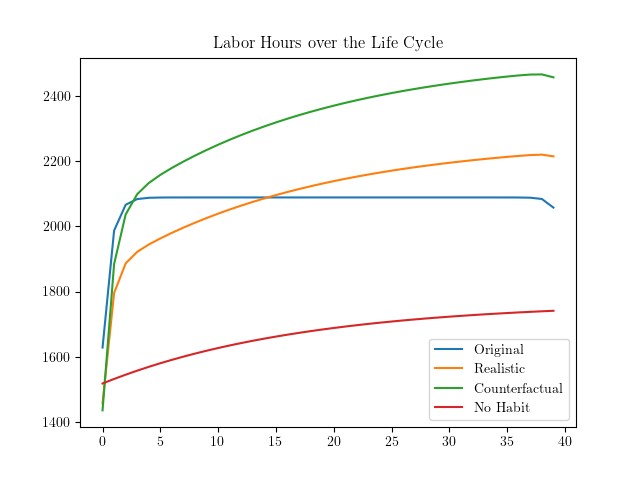
\includegraphics[width=0.8\textwidth]{\FigDir/hours_lc.png}
\end{center}
    \end{frame}

    \begin{frame}
      \frametitle{Elasticities}
      \begin{table}
\centering
\caption{Simulated Elasticities}
\label{tab:elasts}
\begin{tabular}{lrr}
\toprule
{} & $\epsilon$ & $\eta^{\alpha}$ \\
Simulation   &            &                 \\
\midrule
Original     &     0.0734 &         -0.1272 \\
Realistic I  &     0.0658 &         -0.1206 \\
Realsitic II &     0.0776 &         -0.1222 \\
No Habit     &     0.0606 &         -0.1505 \\
\bottomrule
\end{tabular}
\end{table}

      \end{frame}

\begin{frame}

\renewcommand{\bibsection}{\subsubsection*{\bibname }}

\tiny 

\bibliography{\texnameMaster,\econtexBib}

\end{frame}
\end{document}\endinput

% Local Variables:
% eval: (setq TeX-command-list  (remove '("Biber" "biber %s" TeX-run-Biber nil  (plain-tex-mode latex-mode doctex-mode ams-tex-mode texinfo-mode)  :help "Run Biber") TeX-command-list))
% eval: (setq TeX-command-list  (remove '("BibTeX" "%(bibtex) %s" TeX-run-BibTeX nil t                                                                              :help "Run BibTeX") TeX-command-list))
% eval: (setq TeX-command-list  (remove '("BibTeX" "%(bibtex) %s" TeX-run-BibTeX nil (plain-tex-mode latex-mode doctex-mode ams-tex-mode texinfo-mode context-mode) :help "Run BibTeX") TeX-command-list))
% eval: (setq TeX-command-list  (remove '("BibTeX" "%(bibtex) ../LaTeX/%s" TeX-run-BibTeX nil t :help "Run BibTeX")   TeX-command-list))
% eval: (add-to-list 'TeX-command-list	'("BibTeX" "%(bibtex) LaTeX/%s" TeX-run-BibTeX nil t :help "Run BibTeX") t)
% eval: (cond ((string-equal system-type "darwin") (progn (setq TeX-view-program-list '(("Skim" "/Applications/Skim.app/Contents/SharedSupport/displayline -b %n LaTeX/%o %b"))))))
% TeX-PDF-mode: t
% TeX-file-line-error: t
% TeX-debug-warnings: t
% LaTeX-command-style: (("" "%(PDF)%(latex) %(file-line-error) %(extraopts) -output-directory=LaTeX %S%(PDFout)"))
% TeX-source-correlate-mode: t
% TeX-source-correlate-start-server: 0
% TeX-parse-self: t
% End:
